\documentclass[addpoints,12pt]{exam}

\usepackage{amsmath}
\usepackage{amsthm}
\usepackage{graphicx}
\usepackage{enumitem}
\usepackage{amssymb}
\usepackage{tikz}
\usepackage{multicol}
\usepackage{comment}
\usepackage{geometry}
\usepackage{enumitem}
\usepackage{xcolor}
\usepackage{tikz}
\usepackage{hyperref}
\newcommand{\BM}[1]{{\color{red} #1}}

\printanswers %Remove to hide answers
\pagestyle{headandfoot} %Adds Headers and Footers
\runningheadrule
\firstpageheader{Math 125}{Exam 2 }{\today}
\runningheader{Math 125}
{Exam 2, Page \thepage\ of \numpages}
{\today}
\firstpagefooter{}{\thepage}{}
\runningfooter{}{\thepage}{}

\newcommand{\tft}{
\begin{oneparcheckboxes}
\CorrectChoice True
\choice False
	\end{oneparcheckboxes}
}\hypersetup{
    colorlinks=true,
    linkcolor=blue,
    filecolor=magenta,      
    urlcolor=cyan,
    pdftitle={Overleaf Example},
    pdfpagemode=FullScreen,
    }
\newcommand{\tff}{
\begin{oneparcheckboxes}
\choice True
\CorrectChoice False
	\end{oneparcheckboxes}
	
}
\newcommand{\ynn}{
\begin{oneparcheckboxes}
\choice Yes
\CorrectChoice No
	\end{oneparcheckboxes}
}
\newcommand{\yny}{
\begin{oneparcheckboxes}
\CorrectChoice Yes
\choice No 
	\end{oneparcheckboxes}
}
\checkboxchar{$\Box$}
\checkedchar{$\blacksquare$}


\newtheorem{theorem}{Theorem}

\begin{document}

%The box at the top, and the name
\begin{center}
\fbox{\fbox{\parbox{5.5in}{\centering There are $162$ points on this exam. Completing $60$ of them will get you $100\%$ on this exam. You may attempt more than $60$ points. For example, half credit on every question would be answering $81$ points and would recieve an $A$, since it is more than $60$. Several questions have multiple parts to them. Do not feel like you need to do all the parts. For instance, you could only do part $d)$ of one question and no other parts. I will grade this exam harshly, since it is open notes. You may use your book, notes, general math facts found online. If you use other humans or use Chat-GPT or other AI models to complete the exam, you will recieve a $0$ on the exam and there will be no retakes. There will be an oral portion of the exam where I will ask you to go over the answers to the exam out loud as well. I wish you the best of luck, and I hope you have fun with the problems. \textbf{Due:Friday October 31st 5pm }}}}
\end{center}
\vspace{0.1in}
\makebox[\textwidth]{Name:\enspace\hrulefill}
\vspace{0.2in}

%Question Formatting
%\qformat{\textbf{Question \thequestion}\quad (\thepoints)\hfill}
%Point Table

%\begin{center}
%\gradetable[h][questions]
%\end{center}

%Beginning Questions
\begin{questions}
	\question My brother-in-law is building a commodity shed. Let's help him build it! 
	\begin{parts}
		\part[4] He would like to make a rectangular building that is $10$ feet tall. The walls cost $8$ dollars per square foot. He only has budgeted $8000$ dollars for the walls. Write an inequality involving the length and width of the building to ensure that the building stays under budget. 
		\part[8] Assume that the volume must be at least 4000 cubic feet. What is the minimum and maximum length and widths required so that we are within budget, and we have a volume of $4000$ cubic feet? Assume that we also will use all $\$8000$. 
		\part[5] Let length be the $x$ axis and width be the $y$-axis in the plane. Use desmos to visualize all possible values that keep the cost lower than $8000$ while also keeping the volume larger than $4000$ cubic feet. 
		\part[3] Verify that a length of $20$ and a width of $30$ is a valid length for our shed. 
		\part[8] Time to add a roof. Assume that we stick with our $20x30$ measurement for the length and width. The roof is sloped in the direction of the $30$ foot side. Assume that the roof is $19$ feet tall at the tallest point (which is $15$ feet from each wall). There will be $5$ beams evenly spaced that are drawn in blue below. How tall should each of these $5$, beams be? 
			\begin{center}
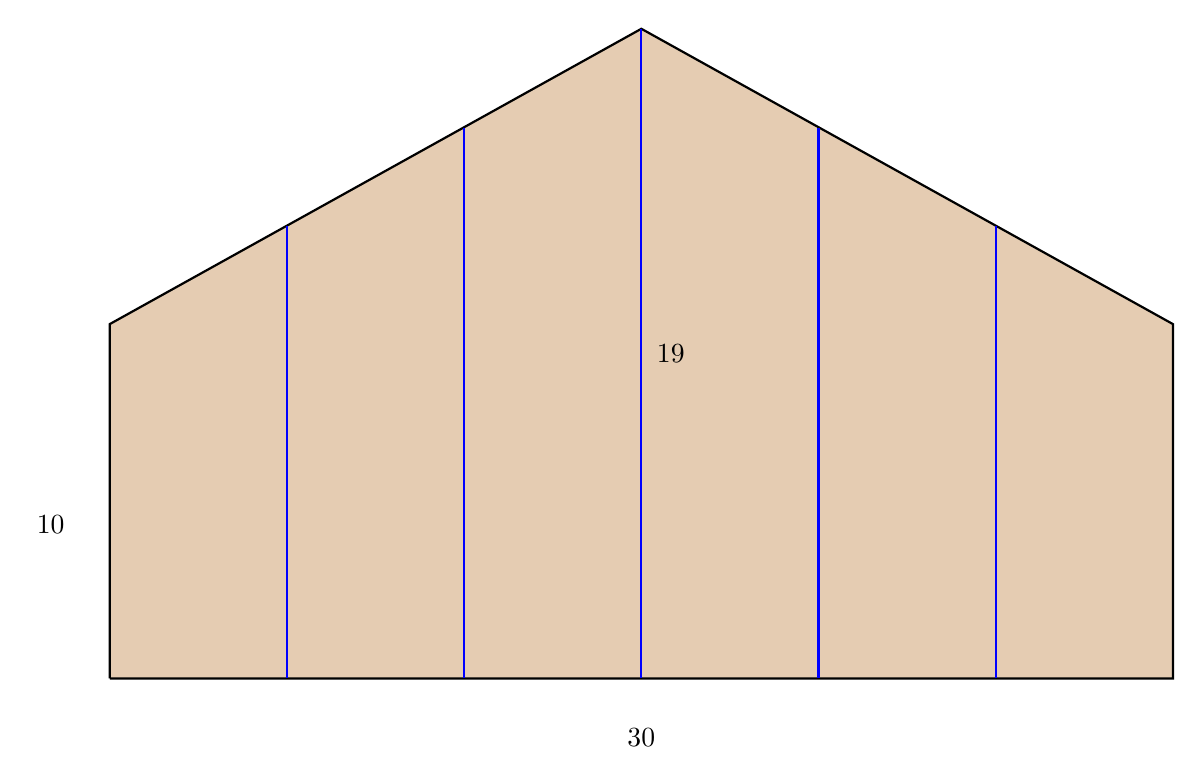
\begin{tikzpicture}[thick, scale=1.5]
    % Define coordinates for key points for easier adjustments
    \coordinate (bottom left) at (0,0);
    \coordinate (top left) at (0,3);
    \coordinate (bottom right) at (9,0);
    \coordinate (top right) at (9,3);
    \coordinate (roof peak) at (4.5,5.5);
		\coordinate (bottom first beam) at (1.5,0) ;
		\coordinate (top first beam) at (1.5,3.83); 
		\coordinate (top second beam) at (3,4.66);
		\coordinate (bottom second beam) at (3,0);
		\coordinate (middle bottom) at (4.5,0); 

		\coordinate (top fourth beam) at (6,4.66);
		\coordinate (bottom fourth beam) at (6,0);
		\coordinate (top fifth beam) at (7.5,3.83);
		\coordinate (bottom fifth beam) at (7.5,0);
    % Ground line

    % Main house body (rectangle)
    % Use coordinates for cleaner code
    \draw[fill=brown!40] (bottom left) -- (bottom right) -- (top right) -- (roof peak)-- (top left) -- (bottom left); 
		\draw[blue] (bottom first beam) -- (top first beam);
		\draw[blue] (bottom second beam) -- (top second beam);
		\draw[blue] (middle bottom) -- (roof peak);
		\draw[blue] (bottom fourth beam) -- (top fourth beam);
		\draw[blue] (bottom fifth beam) -- (top fifth beam);
		\draw (4.75,2.75) node {19};
		\draw (4.5, -0.5) node {30};
		\draw (-0.5,1.3) node {10};
    % Right window
\end{tikzpicture}
\end{center}
	\end{parts}
	\question We are looking to buy a new car. Answer the following questions involved in buying a new car. 
	\begin{parts}
	\part[4] Find a car for sale in Yankton. Provide the info of where you found the car, price, new or used, and as many details as you find relevant about the car. 
	\part[2] Cars typically have different interest rates depending on if the car is new or used. Here is a table of the average auto loan interest rates based on credit scores, and if the car is new or used 
		\[
		\begin{tabular}{|c|c|c|}
			Credit Score & New & Used \\
			\hline
			781-850 & 5.18\% & 6.82\% \\
			\hline
			661-780 & 6.7\% & 9.06 \% \\
			\hline
			601 - 660 & 9.83\% & 13.74\% \\
			\hline
			501-600 & 13.22\% & 18.99\% \\
			\hline
			300-500 & 15.81\% & 21.58\% \\
			\hline
		\end{tabular}
	\]
	    Why are interest rates more for used cars in comparison to new cars, and why would they be more for bad credit scores verses good credit scores? 
		\part[4] For the car you have selected, pick a credit range above. What is the difference in the monthly payments between a $3$ year loan and a $5$ year loan? 
		\part[3] How much more money will you spend overall if you go with the $3$ year loan instead of the $5$ year loan? 
		\part[4] Pick either the $5$ year loan or the $3$ year loan, your choice. Calculate for your car the diffence in monthly payments between a credit score of $800$ and $650$. 
		\part[3] How much more money will you spend overall with the credit score of $650$ instead of $800$?
		\part[6] Assume now that you want to spend no more than $\$400$ a month on a car. Pick a credit score, year length of loan, and if you would like a new or used car. What is the maximum value of a car that you can purchase? 
	\end{parts}
	\question The acceleration due to gravity is $32.2 $ $ft$/$s^{2}$. This means that after $t$ number of seconds, the velocity of something in freefall is given by 
	\[
	v = -32.2 t
	\]
	Where the negative comes from things falling toward the earth. If you would like to have some sort of a starting speed, then the velocity equation becomes 
	\[
	v = -32.2 t +v_0
	\]
	where $v_0$ is the starting speed. $v_0$ is positive if the object is traveling away from earth, and negative if it is falling toward earth. The height of the ball is then given by
	\[
	y = \frac{1}{2}*32.2 t^{2}+v_0t+h_0 = 16.1 t^{2}+v_0t+h
	\]
	\begin{parts}
	\part[8] Throw something up into the air (throw something that avoids air resistance, i.e. don't throw a feather, but also don't hurt anyone, i.e. don't shoot arrows into the air) and time how long it takes $(t)$ to hit the ground $(y=0)$. Be sure to measure the height that you release the object from $(h)$. What is the initial velocity that you threw the object at? 
	\part[6] How far up did the object travel? Hint: The velocity is positive when you throw the object up, and negative when you throw the object down. So what must be the velicity of the object at its peak?
	\part[6] Assume that you throw the ball from $10$ feet higher with the same initial velociy. How much longer will it take for your object to hit the ground. 
	\end{parts}

	\question This problem involves coding. If you are looking for places to start to learn to code, you are able to sign up for the Jetbrains Student Pack and get access to their IDE's. This is a free resource (Normally is over $\$200$). There are lots of other places to write and compile code however, such as Visual Studio, Neovim, Emacs, and so on. All of these are free as well. You should not need to pay to complete this problem. 
	    \begin{parts}
			\part[2] Pick a computer language and print the string $"Hello World"$. Python or Lua are my recommended suggestion for which language to start in. 
			\part[5] Write a function that computes the quadratic formula in the language you have chosen. 
			\part[4] Graph the function $f(x) = x^{2}$ in your language. 
			\part[4] Print the first $1000$ numbers in the pattern 
				\[
				2,4,6,8,10,12,\dots
				\]
			\part[10] Write a function or a program that is useful to you. I will give higher point values depending on the complexity of the program that you write. Some examples could be 
				\begin{itemize}
					\item Make a small website. Doesn't need to be fancy! (Probably need HTML, CSS)
					\item Make the start of a computer game where you move around a circle on a screen. (I suggest looking at Love2D and Lua. This is what the game Balatro was made in. )
					\item Make a to do list app. 
					\item Make your own calculator. 
					\item Generate a fractal using your program. 
					\item Solve the Koch Snowflake Problem. 
				\end{itemize}
	    \end{parts}
			\question[20] Find the area of the Koch Snowflake where you start with a triangle with side length $1$. 
			\question This problem will guide you through finding the following formula. 
			\begin{equation}\label{eq:annuity}
			a+ar+ar^{2}+ar^{3}+ar^{4}+\dots +ar^{n-1} =  a \frac{1-r^{n}}{1-r}
			\end{equation}
			This formula is used in both the car and housing payments, as well as used in calculating investments, Koch Snowflake, and lots of other areas of life. 
			\begin{parts}
			\part[7] Assume you would like to start saving money into an account the collects compount interest at a rate $r$, where your interest is compounded $n$ times a year over $t$ years. You payments ($PMT$) in each time that the interest is compounded, and so after $t$ years you have 
			\[
					PMT + PMT(1+\frac{r}{n}) + PMT \left(1+\frac{r}{n}\right)^{2} + \dots + PMT\left(1+\frac{r}{n}\right)^{nt-1}
					\]
				into your account. 	Use the formula (\ref{eq:annuity}) above to calculate how much is in your account. Compare with the annuity formula in your book (Section 8.5). 
			\part[6] Assume that your payments are $1000$ dollars monthly into an account that pays $8\%$ interest. How much do you have after $4$ years? 
			\part[1] We now seek to derive the formula (\ref{eq:annuity}) above. What do you get when you multiply
				\[
					(1)(a+ar+ar^{2}+ar^{3}+\dots +ar^{n-1})= 
				\]
			\part[3]What do you get when you multiply 
				\[
				-r(a+ar+ar^{2}+\dots +ar^{n-1}) = 
				\]
			\part[5]What do you get when you multiply 
				\[
					(1-r)(a+ar+ar^{2}+\dots +ar^{n-1}) = 
				\]
			\part[2]Why are these two things equal? 
				\[
					\left(\frac{1-r}{1-r}\right)(a+ar+ar^{2}+\dots +ar^{n-1}) = (a+ar+ar^{2}+\dots+ar^{n})
				\]
			\part[8] Using Part e), show that 
				\[
				\left(\frac{1-r}{1-r}\right)(a+ar+ar^{2}+\dots +ar^{n-1}) = a\frac{1-r^{n}}{1-r}
				\]

			\end{parts}
	\question[10] If you write your exam using Latex, you get $10$ bonus points. A good resource to get started and to write Latex is \href{www.overleaf.com}{www.overleaf.com}. 
	\question[1] Pretend you get to create a triathalon where you get to pick three events. These events do not need to be in any way athletic. What 3 events would you choose so that you were the best in the world at that triathlon? For example, my 3 would be: $\infty$-categories (Math), dairy farming, and archery. 
\end{questions}

    
\end{document}

